\documentclass[11pt]{article}

    \usepackage{biblatex}
    \addbibresource{bibliography.bib}
    \usepackage[breakable]{tcolorbox}
    \usepackage{parskip} % Stop auto-indenting (to mimic markdown behaviour)
    
    \usepackage{iftex}
    \ifPDFTeX
    	\usepackage[T1]{fontenc}
    	\usepackage{mathpazo}
    \else
    	\usepackage{fontspec}
    \fi
    

    % Basic figure setup, for now with no caption control since it's done
    % automatically by Pandoc (which extracts ![](path) syntax from Markdown).
    \usepackage{graphicx}
    % Maintain compatibility with old templates. Remove in nbconvert 6.0
    \let\Oldincludegraphics\includegraphics
    % Ensure that by default, figures have no caption (until we provide a
    % proper Figure object with a Caption API and a way to capture that
    % in the conversion process - todo).
    \usepackage{caption}
    \DeclareCaptionFormat{nocaption}{}
    \captionsetup{format=nocaption,aboveskip=0pt,belowskip=0pt}

    \usepackage[Export]{adjustbox} % Used to constrain images to a maximum size
    \adjustboxset{max size={0.9\linewidth}{0.9\paperheight}}
    \usepackage{float}
    \floatplacement{figure}{H} % forces figures to be placed at the correct location
    \usepackage{xcolor} % Allow colors to be defined
    \usepackage{enumerate} % Needed for markdown enumerations to work
    \usepackage{geometry} % Used to adjust the document margins
    \usepackage{amsmath} % Equations
    \usepackage{amssymb} % Equations
    \usepackage{textcomp} % defines textquotesingle
    % Hack from http://tex.stackexchange.com/a/47451/13684:
    \AtBeginDocument{%
        \def\PYZsq{\textquotesingle}% Upright quotes in Pygmentized code
    }
    \usepackage{upquote} % Upright quotes for verbatim code
    \usepackage{eurosym} % defines \euro
    \usepackage[mathletters]{ucs} % Extended unicode (utf-8) support
    \usepackage{fancyvrb} % verbatim replacement that allows latex

    % The hyperref package gives us a pdf with properly built
    % internal navigation ('pdf bookmarks' for the table of contents,
    % internal cross-reference links, web links for URLs, etc.)
    \usepackage{hyperref}
    % The default LaTeX title has an obnoxious amount of whitespace. By default,
    % titling removes some of it. It also provides customization options.
    \usepackage{titling}
    \usepackage{longtable} % longtable support required by pandoc >1.10
    \usepackage{booktabs}  % table support for pandoc > 1.12.2
    \usepackage[inline]{enumitem} % IRkernel/repr support (it uses the enumerate* environment)
    \usepackage[normalem]{ulem} % ulem is needed to support strikethroughs (\sout)
                                % normalem makes italics be italics, not underlines
    \usepackage{mathrsfs}
    

    
    % Colors for the hyperref package
    \definecolor{urlcolor}{rgb}{0,.145,.698}
    \definecolor{linkcolor}{rgb}{.71,0.21,0.01}
    \definecolor{citecolor}{rgb}{.12,.54,.11}

    % ANSI colors
    \definecolor{ansi-black}{HTML}{3E424D}
    \definecolor{ansi-black-intense}{HTML}{282C36}
    \definecolor{ansi-red}{HTML}{E75C58}
    \definecolor{ansi-red-intense}{HTML}{B22B31}
    \definecolor{ansi-green}{HTML}{00A250}
    \definecolor{ansi-green-intense}{HTML}{007427}
    \definecolor{ansi-yellow}{HTML}{DDB62B}
    \definecolor{ansi-yellow-intense}{HTML}{B27D12}
    \definecolor{ansi-blue}{HTML}{208FFB}
    \definecolor{ansi-blue-intense}{HTML}{0065CA}
    \definecolor{ansi-magenta}{HTML}{D160C4}
    \definecolor{ansi-magenta-intense}{HTML}{A03196}
    \definecolor{ansi-cyan}{HTML}{60C6C8}
    \definecolor{ansi-cyan-intense}{HTML}{258F8F}
    \definecolor{ansi-white}{HTML}{C5C1B4}
    \definecolor{ansi-white-intense}{HTML}{A1A6B2}
    \definecolor{ansi-default-inverse-fg}{HTML}{FFFFFF}
    \definecolor{ansi-default-inverse-bg}{HTML}{000000}

    % commands and environments needed by pandoc snippets
    % extracted from the output of `pandoc -s`
    \providecommand{\tightlist}{%
      \setlength{\itemsep}{0pt}\setlength{\parskip}{0pt}}
    \DefineVerbatimEnvironment{Highlighting}{Verbatim}{commandchars=\\\{\}}
    % Add ',fontsize=\small' for more characters per line
    \newenvironment{Shaded}{}{}
    \newcommand{\KeywordTok}[1]{\textcolor[rgb]{0.00,0.44,0.13}{\textbf{{#1}}}}
    \newcommand{\DataTypeTok}[1]{\textcolor[rgb]{0.56,0.13,0.00}{{#1}}}
    \newcommand{\DecValTok}[1]{\textcolor[rgb]{0.25,0.63,0.44}{{#1}}}
    \newcommand{\BaseNTok}[1]{\textcolor[rgb]{0.25,0.63,0.44}{{#1}}}
    \newcommand{\FloatTok}[1]{\textcolor[rgb]{0.25,0.63,0.44}{{#1}}}
    \newcommand{\CharTok}[1]{\textcolor[rgb]{0.25,0.44,0.63}{{#1}}}
    \newcommand{\StringTok}[1]{\textcolor[rgb]{0.25,0.44,0.63}{{#1}}}
    \newcommand{\CommentTok}[1]{\textcolor[rgb]{0.38,0.63,0.69}{\textit{{#1}}}}
    \newcommand{\OtherTok}[1]{\textcolor[rgb]{0.00,0.44,0.13}{{#1}}}
    \newcommand{\AlertTok}[1]{\textcolor[rgb]{1.00,0.00,0.00}{\textbf{{#1}}}}
    \newcommand{\FunctionTok}[1]{\textcolor[rgb]{0.02,0.16,0.49}{{#1}}}
    \newcommand{\RegionMarkerTok}[1]{{#1}}
    \newcommand{\ErrorTok}[1]{\textcolor[rgb]{1.00,0.00,0.00}{\textbf{{#1}}}}
    \newcommand{\NormalTok}[1]{{#1}}
    
    % Additional commands for more recent versions of Pandoc
    \newcommand{\ConstantTok}[1]{\textcolor[rgb]{0.53,0.00,0.00}{{#1}}}
    \newcommand{\SpecialCharTok}[1]{\textcolor[rgb]{0.25,0.44,0.63}{{#1}}}
    \newcommand{\VerbatimStringTok}[1]{\textcolor[rgb]{0.25,0.44,0.63}{{#1}}}
    \newcommand{\SpecialStringTok}[1]{\textcolor[rgb]{0.73,0.40,0.53}{{#1}}}
    \newcommand{\ImportTok}[1]{{#1}}
    \newcommand{\DocumentationTok}[1]{\textcolor[rgb]{0.73,0.13,0.13}{\textit{{#1}}}}
    \newcommand{\AnnotationTok}[1]{\textcolor[rgb]{0.38,0.63,0.69}{\textbf{\textit{{#1}}}}}
    \newcommand{\CommentVarTok}[1]{\textcolor[rgb]{0.38,0.63,0.69}{\textbf{\textit{{#1}}}}}
    \newcommand{\VariableTok}[1]{\textcolor[rgb]{0.10,0.09,0.49}{{#1}}}
    \newcommand{\ControlFlowTok}[1]{\textcolor[rgb]{0.00,0.44,0.13}{\textbf{{#1}}}}
    \newcommand{\OperatorTok}[1]{\textcolor[rgb]{0.40,0.40,0.40}{{#1}}}
    \newcommand{\BuiltInTok}[1]{{#1}}
    \newcommand{\ExtensionTok}[1]{{#1}}
    \newcommand{\PreprocessorTok}[1]{\textcolor[rgb]{0.74,0.48,0.00}{{#1}}}
    \newcommand{\AttributeTok}[1]{\textcolor[rgb]{0.49,0.56,0.16}{{#1}}}
    \newcommand{\InformationTok}[1]{\textcolor[rgb]{0.38,0.63,0.69}{\textbf{\textit{{#1}}}}}
    \newcommand{\WarningTok}[1]{\textcolor[rgb]{0.38,0.63,0.69}{\textbf{\textit{{#1}}}}}
    
    
    % Define a nice break command that doesn't care if a line doesn't already
    % exist.
    \def\br{\hspace*{\fill} \\* }
    % Math Jax compatibility definitions
    \def\gt{>}
    \def\lt{<}
    \let\Oldtex\TeX
    \let\Oldlatex\LaTeX
    \renewcommand{\TeX}{\textrm{\Oldtex}}
    \renewcommand{\LaTeX}{\textrm{\Oldlatex}}
    % Document parameters
    % Document title
    \title{Covid-19 Analysis}
    
    
    
    
    
% Pygments definitions
\makeatletter
\def\PY@reset{\let\PY@it=\relax \let\PY@bf=\relax%
    \let\PY@ul=\relax \let\PY@tc=\relax%
    \let\PY@bc=\relax \let\PY@ff=\relax}
\def\PY@tok#1{\csname PY@tok@#1\endcsname}
\def\PY@toks#1+{\ifx\relax#1\empty\else%
    \PY@tok{#1}\expandafter\PY@toks\fi}
\def\PY@do#1{\PY@bc{\PY@tc{\PY@ul{%
    \PY@it{\PY@bf{\PY@ff{#1}}}}}}}
\def\PY#1#2{\PY@reset\PY@toks#1+\relax+\PY@do{#2}}

\expandafter\def\csname PY@tok@w\endcsname{\def\PY@tc##1{\textcolor[rgb]{0.73,0.73,0.73}{##1}}}
\expandafter\def\csname PY@tok@c\endcsname{\let\PY@it=\textit\def\PY@tc##1{\textcolor[rgb]{0.25,0.50,0.50}{##1}}}
\expandafter\def\csname PY@tok@cp\endcsname{\def\PY@tc##1{\textcolor[rgb]{0.74,0.48,0.00}{##1}}}
\expandafter\def\csname PY@tok@k\endcsname{\let\PY@bf=\textbf\def\PY@tc##1{\textcolor[rgb]{0.00,0.50,0.00}{##1}}}
\expandafter\def\csname PY@tok@kp\endcsname{\def\PY@tc##1{\textcolor[rgb]{0.00,0.50,0.00}{##1}}}
\expandafter\def\csname PY@tok@kt\endcsname{\def\PY@tc##1{\textcolor[rgb]{0.69,0.00,0.25}{##1}}}
\expandafter\def\csname PY@tok@o\endcsname{\def\PY@tc##1{\textcolor[rgb]{0.40,0.40,0.40}{##1}}}
\expandafter\def\csname PY@tok@ow\endcsname{\let\PY@bf=\textbf\def\PY@tc##1{\textcolor[rgb]{0.67,0.13,1.00}{##1}}}
\expandafter\def\csname PY@tok@nb\endcsname{\def\PY@tc##1{\textcolor[rgb]{0.00,0.50,0.00}{##1}}}
\expandafter\def\csname PY@tok@nf\endcsname{\def\PY@tc##1{\textcolor[rgb]{0.00,0.00,1.00}{##1}}}
\expandafter\def\csname PY@tok@nc\endcsname{\let\PY@bf=\textbf\def\PY@tc##1{\textcolor[rgb]{0.00,0.00,1.00}{##1}}}
\expandafter\def\csname PY@tok@nn\endcsname{\let\PY@bf=\textbf\def\PY@tc##1{\textcolor[rgb]{0.00,0.00,1.00}{##1}}}
\expandafter\def\csname PY@tok@ne\endcsname{\let\PY@bf=\textbf\def\PY@tc##1{\textcolor[rgb]{0.82,0.25,0.23}{##1}}}
\expandafter\def\csname PY@tok@nv\endcsname{\def\PY@tc##1{\textcolor[rgb]{0.10,0.09,0.49}{##1}}}
\expandafter\def\csname PY@tok@no\endcsname{\def\PY@tc##1{\textcolor[rgb]{0.53,0.00,0.00}{##1}}}
\expandafter\def\csname PY@tok@nl\endcsname{\def\PY@tc##1{\textcolor[rgb]{0.63,0.63,0.00}{##1}}}
\expandafter\def\csname PY@tok@ni\endcsname{\let\PY@bf=\textbf\def\PY@tc##1{\textcolor[rgb]{0.60,0.60,0.60}{##1}}}
\expandafter\def\csname PY@tok@na\endcsname{\def\PY@tc##1{\textcolor[rgb]{0.49,0.56,0.16}{##1}}}
\expandafter\def\csname PY@tok@nt\endcsname{\let\PY@bf=\textbf\def\PY@tc##1{\textcolor[rgb]{0.00,0.50,0.00}{##1}}}
\expandafter\def\csname PY@tok@nd\endcsname{\def\PY@tc##1{\textcolor[rgb]{0.67,0.13,1.00}{##1}}}
\expandafter\def\csname PY@tok@s\endcsname{\def\PY@tc##1{\textcolor[rgb]{0.73,0.13,0.13}{##1}}}
\expandafter\def\csname PY@tok@sd\endcsname{\let\PY@it=\textit\def\PY@tc##1{\textcolor[rgb]{0.73,0.13,0.13}{##1}}}
\expandafter\def\csname PY@tok@si\endcsname{\let\PY@bf=\textbf\def\PY@tc##1{\textcolor[rgb]{0.73,0.40,0.53}{##1}}}
\expandafter\def\csname PY@tok@se\endcsname{\let\PY@bf=\textbf\def\PY@tc##1{\textcolor[rgb]{0.73,0.40,0.13}{##1}}}
\expandafter\def\csname PY@tok@sr\endcsname{\def\PY@tc##1{\textcolor[rgb]{0.73,0.40,0.53}{##1}}}
\expandafter\def\csname PY@tok@ss\endcsname{\def\PY@tc##1{\textcolor[rgb]{0.10,0.09,0.49}{##1}}}
\expandafter\def\csname PY@tok@sx\endcsname{\def\PY@tc##1{\textcolor[rgb]{0.00,0.50,0.00}{##1}}}
\expandafter\def\csname PY@tok@m\endcsname{\def\PY@tc##1{\textcolor[rgb]{0.40,0.40,0.40}{##1}}}
\expandafter\def\csname PY@tok@gh\endcsname{\let\PY@bf=\textbf\def\PY@tc##1{\textcolor[rgb]{0.00,0.00,0.50}{##1}}}
\expandafter\def\csname PY@tok@gu\endcsname{\let\PY@bf=\textbf\def\PY@tc##1{\textcolor[rgb]{0.50,0.00,0.50}{##1}}}
\expandafter\def\csname PY@tok@gd\endcsname{\def\PY@tc##1{\textcolor[rgb]{0.63,0.00,0.00}{##1}}}
\expandafter\def\csname PY@tok@gi\endcsname{\def\PY@tc##1{\textcolor[rgb]{0.00,0.63,0.00}{##1}}}
\expandafter\def\csname PY@tok@gr\endcsname{\def\PY@tc##1{\textcolor[rgb]{1.00,0.00,0.00}{##1}}}
\expandafter\def\csname PY@tok@ge\endcsname{\let\PY@it=\textit}
\expandafter\def\csname PY@tok@gs\endcsname{\let\PY@bf=\textbf}
\expandafter\def\csname PY@tok@gp\endcsname{\let\PY@bf=\textbf\def\PY@tc##1{\textcolor[rgb]{0.00,0.00,0.50}{##1}}}
\expandafter\def\csname PY@tok@go\endcsname{\def\PY@tc##1{\textcolor[rgb]{0.53,0.53,0.53}{##1}}}
\expandafter\def\csname PY@tok@gt\endcsname{\def\PY@tc##1{\textcolor[rgb]{0.00,0.27,0.87}{##1}}}
\expandafter\def\csname PY@tok@err\endcsname{\def\PY@bc##1{\setlength{\fboxsep}{0pt}\fcolorbox[rgb]{1.00,0.00,0.00}{1,1,1}{\strut ##1}}}
\expandafter\def\csname PY@tok@kc\endcsname{\let\PY@bf=\textbf\def\PY@tc##1{\textcolor[rgb]{0.00,0.50,0.00}{##1}}}
\expandafter\def\csname PY@tok@kd\endcsname{\let\PY@bf=\textbf\def\PY@tc##1{\textcolor[rgb]{0.00,0.50,0.00}{##1}}}
\expandafter\def\csname PY@tok@kn\endcsname{\let\PY@bf=\textbf\def\PY@tc##1{\textcolor[rgb]{0.00,0.50,0.00}{##1}}}
\expandafter\def\csname PY@tok@kr\endcsname{\let\PY@bf=\textbf\def\PY@tc##1{\textcolor[rgb]{0.00,0.50,0.00}{##1}}}
\expandafter\def\csname PY@tok@bp\endcsname{\def\PY@tc##1{\textcolor[rgb]{0.00,0.50,0.00}{##1}}}
\expandafter\def\csname PY@tok@fm\endcsname{\def\PY@tc##1{\textcolor[rgb]{0.00,0.00,1.00}{##1}}}
\expandafter\def\csname PY@tok@vc\endcsname{\def\PY@tc##1{\textcolor[rgb]{0.10,0.09,0.49}{##1}}}
\expandafter\def\csname PY@tok@vg\endcsname{\def\PY@tc##1{\textcolor[rgb]{0.10,0.09,0.49}{##1}}}
\expandafter\def\csname PY@tok@vi\endcsname{\def\PY@tc##1{\textcolor[rgb]{0.10,0.09,0.49}{##1}}}
\expandafter\def\csname PY@tok@vm\endcsname{\def\PY@tc##1{\textcolor[rgb]{0.10,0.09,0.49}{##1}}}
\expandafter\def\csname PY@tok@sa\endcsname{\def\PY@tc##1{\textcolor[rgb]{0.73,0.13,0.13}{##1}}}
\expandafter\def\csname PY@tok@sb\endcsname{\def\PY@tc##1{\textcolor[rgb]{0.73,0.13,0.13}{##1}}}
\expandafter\def\csname PY@tok@sc\endcsname{\def\PY@tc##1{\textcolor[rgb]{0.73,0.13,0.13}{##1}}}
\expandafter\def\csname PY@tok@dl\endcsname{\def\PY@tc##1{\textcolor[rgb]{0.73,0.13,0.13}{##1}}}
\expandafter\def\csname PY@tok@s2\endcsname{\def\PY@tc##1{\textcolor[rgb]{0.73,0.13,0.13}{##1}}}
\expandafter\def\csname PY@tok@sh\endcsname{\def\PY@tc##1{\textcolor[rgb]{0.73,0.13,0.13}{##1}}}
\expandafter\def\csname PY@tok@s1\endcsname{\def\PY@tc##1{\textcolor[rgb]{0.73,0.13,0.13}{##1}}}
\expandafter\def\csname PY@tok@mb\endcsname{\def\PY@tc##1{\textcolor[rgb]{0.40,0.40,0.40}{##1}}}
\expandafter\def\csname PY@tok@mf\endcsname{\def\PY@tc##1{\textcolor[rgb]{0.40,0.40,0.40}{##1}}}
\expandafter\def\csname PY@tok@mh\endcsname{\def\PY@tc##1{\textcolor[rgb]{0.40,0.40,0.40}{##1}}}
\expandafter\def\csname PY@tok@mi\endcsname{\def\PY@tc##1{\textcolor[rgb]{0.40,0.40,0.40}{##1}}}
\expandafter\def\csname PY@tok@il\endcsname{\def\PY@tc##1{\textcolor[rgb]{0.40,0.40,0.40}{##1}}}
\expandafter\def\csname PY@tok@mo\endcsname{\def\PY@tc##1{\textcolor[rgb]{0.40,0.40,0.40}{##1}}}
\expandafter\def\csname PY@tok@ch\endcsname{\let\PY@it=\textit\def\PY@tc##1{\textcolor[rgb]{0.25,0.50,0.50}{##1}}}
\expandafter\def\csname PY@tok@cm\endcsname{\let\PY@it=\textit\def\PY@tc##1{\textcolor[rgb]{0.25,0.50,0.50}{##1}}}
\expandafter\def\csname PY@tok@cpf\endcsname{\let\PY@it=\textit\def\PY@tc##1{\textcolor[rgb]{0.25,0.50,0.50}{##1}}}
\expandafter\def\csname PY@tok@c1\endcsname{\let\PY@it=\textit\def\PY@tc##1{\textcolor[rgb]{0.25,0.50,0.50}{##1}}}
\expandafter\def\csname PY@tok@cs\endcsname{\let\PY@it=\textit\def\PY@tc##1{\textcolor[rgb]{0.25,0.50,0.50}{##1}}}

\def\PYZbs{\char`\\}
\def\PYZus{\char`\_}
\def\PYZob{\char`\{}
\def\PYZcb{\char`\}}
\def\PYZca{\char`\^}
\def\PYZam{\char`\&}
\def\PYZlt{\char`\<}
\def\PYZgt{\char`\>}
\def\PYZsh{\char`\#}
\def\PYZpc{\char`\%}
\def\PYZdl{\char`\$}
\def\PYZhy{\char`\-}
\def\PYZsq{\char`\'}
\def\PYZdq{\char`\"}
\def\PYZti{\char`\~}
% for compatibility with earlier versions
\def\PYZat{@}
\def\PYZlb{[}
\def\PYZrb{]}
\makeatother


    % For linebreaks inside Verbatim environment from package fancyvrb. 
    \makeatletter
        \newbox\Wrappedcontinuationbox 
        \newbox\Wrappedvisiblespacebox 
        \newcommand*\Wrappedvisiblespace {\textcolor{red}{\textvisiblespace}} 
        \newcommand*\Wrappedcontinuationsymbol {\textcolor{red}{\llap{\tiny$\m@th\hookrightarrow$}}} 
        \newcommand*\Wrappedcontinuationindent {3ex } 
        \newcommand*\Wrappedafterbreak {\kern\Wrappedcontinuationindent\copy\Wrappedcontinuationbox} 
        % Take advantage of the already applied Pygments mark-up to insert 
        % potential linebreaks for TeX processing. 
        %        {, <, #, %, $, ' and ": go to next line. 
        %        _, }, ^, &, >, - and ~: stay at end of broken line. 
        % Use of \textquotesingle for straight quote. 
        \newcommand*\Wrappedbreaksatspecials {% 
            \def\PYGZus{\discretionary{\char`\_}{\Wrappedafterbreak}{\char`\_}}% 
            \def\PYGZob{\discretionary{}{\Wrappedafterbreak\char`\{}{\char`\{}}% 
            \def\PYGZcb{\discretionary{\char`\}}{\Wrappedafterbreak}{\char`\}}}% 
            \def\PYGZca{\discretionary{\char`\^}{\Wrappedafterbreak}{\char`\^}}% 
            \def\PYGZam{\discretionary{\char`\&}{\Wrappedafterbreak}{\char`\&}}% 
            \def\PYGZlt{\discretionary{}{\Wrappedafterbreak\char`\<}{\char`\<}}% 
            \def\PYGZgt{\discretionary{\char`\>}{\Wrappedafterbreak}{\char`\>}}% 
            \def\PYGZsh{\discretionary{}{\Wrappedafterbreak\char`\#}{\char`\#}}% 
            \def\PYGZpc{\discretionary{}{\Wrappedafterbreak\char`\%}{\char`\%}}% 
            \def\PYGZdl{\discretionary{}{\Wrappedafterbreak\char`\$}{\char`\$}}% 
            \def\PYGZhy{\discretionary{\char`\-}{\Wrappedafterbreak}{\char`\-}}% 
            \def\PYGZsq{\discretionary{}{\Wrappedafterbreak\textquotesingle}{\textquotesingle}}% 
            \def\PYGZdq{\discretionary{}{\Wrappedafterbreak\char`\"}{\char`\"}}% 
            \def\PYGZti{\discretionary{\char`\~}{\Wrappedafterbreak}{\char`\~}}% 
        } 
        % Some characters . , ; ? ! / are not pygmentized. 
        % This macro makes them "active" and they will insert potential linebreaks 
        \newcommand*\Wrappedbreaksatpunct {% 
            \lccode`\~`\.\lowercase{\def~}{\discretionary{\hbox{\char`\.}}{\Wrappedafterbreak}{\hbox{\char`\.}}}% 
            \lccode`\~`\,\lowercase{\def~}{\discretionary{\hbox{\char`\,}}{\Wrappedafterbreak}{\hbox{\char`\,}}}% 
            \lccode`\~`\;\lowercase{\def~}{\discretionary{\hbox{\char`\;}}{\Wrappedafterbreak}{\hbox{\char`\;}}}% 
            \lccode`\~`\:\lowercase{\def~}{\discretionary{\hbox{\char`\:}}{\Wrappedafterbreak}{\hbox{\char`\:}}}% 
            \lccode`\~`\?\lowercase{\def~}{\discretionary{\hbox{\char`\?}}{\Wrappedafterbreak}{\hbox{\char`\?}}}% 
            \lccode`\~`\!\lowercase{\def~}{\discretionary{\hbox{\char`\!}}{\Wrappedafterbreak}{\hbox{\char`\!}}}% 
            \lccode`\~`\/\lowercase{\def~}{\discretionary{\hbox{\char`\/}}{\Wrappedafterbreak}{\hbox{\char`\/}}}% 
            \catcode`\.\active
            \catcode`\,\active 
            \catcode`\;\active
            \catcode`\:\active
            \catcode`\?\active
            \catcode`\!\active
            \catcode`\/\active 
            \lccode`\~`\~ 	
        }
    \makeatother

    \let\OriginalVerbatim=\Verbatim
    \makeatletter
    \renewcommand{\Verbatim}[1][1]{%
        %\parskip\z@skip
        \sbox\Wrappedcontinuationbox {\Wrappedcontinuationsymbol}%
        \sbox\Wrappedvisiblespacebox {\FV@SetupFont\Wrappedvisiblespace}%
        \def\FancyVerbFormatLine ##1{\hsize\linewidth
            \vtop{\raggedright\hyphenpenalty\z@\exhyphenpenalty\z@
                \doublehyphendemerits\z@\finalhyphendemerits\z@
                \strut ##1\strut}%
        }%
        % If the linebreak is at a space, the latter will be displayed as visible
        % space at end of first line, and a continuation symbol starts next line.
        % Stretch/shrink are however usually zero for typewriter font.
        \def\FV@Space {%
            \nobreak\hskip\z@ plus\fontdimen3\font minus\fontdimen4\font
            \discretionary{\copy\Wrappedvisiblespacebox}{\Wrappedafterbreak}
            {\kern\fontdimen2\font}%
        }%
        
        % Allow breaks at special characters using \PYG... macros.
        \Wrappedbreaksatspecials
        % Breaks at punctuation characters . , ; ? ! and / need catcode=\active 	
        \OriginalVerbatim[#1,codes*=\Wrappedbreaksatpunct]%
    }
    \makeatother

    % Exact colors from NB
    \definecolor{incolor}{HTML}{303F9F}
    \definecolor{outcolor}{HTML}{D84315}
    \definecolor{cellborder}{HTML}{CFCFCF}
    \definecolor{cellbackground}{HTML}{F7F7F7}
    
    % prompt
    \makeatletter
    \newcommand{\boxspacing}{\kern\kvtcb@left@rule\kern\kvtcb@boxsep}
    \makeatother
    \newcommand{\prompt}[4]{
        \ttfamily\llap{{\color{#2}[#3]:\hspace{3pt}#4}}\vspace{-\baselineskip}
    }
    

    
    % Prevent overflowing lines due to hard-to-break entities
    \sloppy 
    % Setup hyperref package
    \hypersetup{
      breaklinks=true,  % so long urls are correctly broken across lines
      colorlinks=true,
      urlcolor=urlcolor,
      linkcolor=linkcolor,
      citecolor=citecolor,
      }
    % Slightly bigger margins than the latex defaults
    
    \geometry{verbose,tmargin=1in,bmargin=1in,lmargin=1in,rmargin=1in}
    
\begin{document}

%%%%%%%%%%%%%%%%%%%%%%%%%%%%%%%%%%%%%%%%%%%%%%%%%%%%%%%%%%%%%%%%%%%%%%%%%%%%%%%%%%%%%%%%%

\begin{titlepage}
	\centering
    \vspace*{0.5 cm}
    
\includegraphics[scale = 1]{imgs/Logo-unifi.jpg}\\[1.0 cm]

	\rule{\linewidth}{0.2 mm} \\[0.4 cm]
	{ \huge \bfseries \thetitle}\\
	\rule{\linewidth}{0.2 mm} \\[1 cm]

	\textsc{\large Advanced Algorithms and Graph Mining}\\[5 cm]
	\begin{minipage}{0.5\textwidth}
		\begin{flushleft} \large
			\emph{Professors:}\\
			Marino Andrea\\
			Nocentini Massimo\\
            		%\normalsize{Info su\\
            		%dipartimento\\
            		%del docente}\\
			\end{flushleft}
			\end{minipage}~
			\begin{minipage}{0.4\textwidth}
        
		\begin{flushright} \large
			\emph{Students:} \\
			Chaudhry Abdullah\\
			Raffaelli Claudia\\
		\end{flushright}
        
	\end{minipage}\\[0.1 cm]
	
	\vspace*{2.6 cm}
	\begin{center} \large
			AY 2019 - 2020
		\end{center}

	
\end{titlepage}

%%%%%%%%%%%%%%%%%%%%%%%%%%%%%%%%%%%%%%%%%%%%%%%%%%%%%%%%%%%%%%%%%%%%%%%%%%%%%%%%%%%%%%%%%

\tableofcontents

\section{Abstract}\\
These slides describe a technique to calculate the Betweenness
Centrality of a graph's nodes using Bellman-Ford's algorithm

    \begin{tcolorbox}[breakable, size=fbox, boxrule=1pt, pad at break*=1mm,colback=cellbackground, colframe=cellborder]
\prompt{In}{incolor}{1}{\boxspacing}
\begin{Verbatim}[commandchars=\\\{\}]
\PY{n}{\PYZus{}\PYZus{}AUTHORS\PYZus{}\PYZus{}} \PY{o}{=} \PY{p}{\PYZob{}}\PY{l+s+s1}{\PYZsq{}}\PY{l+s+s1}{ac}\PY{l+s+s1}{\PYZsq{}}\PY{p}{:} \PY{p}{(}\PY{l+s+s2}{\PYZdq{}}\PY{l+s+s2}{Abdullah Chaudhry}\PY{l+s+s2}{\PYZdq{}}\PY{p}{,} 
                      \PY{l+s+s2}{\PYZdq{}}\PY{l+s+s2}{abdullah.chaudhry@stud.unifi.it}\PY{l+s+s2}{\PYZdq{}}\PY{p}{,}
                      \PY{l+s+s2}{\PYZdq{}}\PY{l+s+s2}{https://github.com/chabdullah}\PY{l+s+s2}{\PYZdq{}}\PY{p}{)}\PY{p}{,}
               \PY{l+s+s1}{\PYZsq{}}\PY{l+s+s1}{cr}\PY{l+s+s1}{\PYZsq{}}\PY{p}{:} \PY{p}{(}\PY{l+s+s2}{\PYZdq{}}\PY{l+s+s2}{Claudia Raffaelli}\PY{l+s+s2}{\PYZdq{}}\PY{p}{,} 
                      \PY{l+s+s2}{\PYZdq{}}\PY{l+s+s2}{claudia.raffaelli@stud.unifi.it}\PY{l+s+s2}{\PYZdq{}}\PY{p}{,} 
                      \PY{l+s+s2}{\PYZdq{}}\PY{l+s+s2}{https://github.com/ClaudiaRaffaelli}\PY{l+s+s2}{\PYZdq{}}\PY{p}{,}\PY{p}{)}\PY{p}{\PYZcb{}}

\PY{n}{\PYZus{}\PYZus{}KEYWORDS\PYZus{}\PYZus{}} \PY{o}{=} \PY{p}{[}\PY{l+s+s1}{\PYZsq{}}\PY{l+s+s1}{Python}\PY{l+s+s1}{\PYZsq{}}\PY{p}{,} \PY{l+s+s1}{\PYZsq{}}\PY{l+s+s1}{Jupyter}\PY{l+s+s1}{\PYZsq{}}\PY{p}{,} \PY{l+s+s1}{\PYZsq{}}\PY{l+s+s1}{notebooks}\PY{l+s+s1}{\PYZsq{}}\PY{p}{,} \PY{l+s+s1}{\PYZsq{}}\PY{l+s+s1}{Bellman\PYZhy{}Ford}\PY{l+s+s1}{\PYZsq{}}\PY{p}{,} \PY{l+s+s1}{\PYZsq{}}\PY{l+s+s1}{Betweenness\PYZhy{}Centrality}\PY{l+s+s1}{\PYZsq{}}\PY{p}{,} \PY{l+s+s1}{\PYZsq{}}\PY{l+s+s1}{graphs}\PY{l+s+s1}{\PYZsq{}}\PY{p}{]}
\end{Verbatim}
\end{tcolorbox}

\begin{figure}[h]

\includegraphics[scale=1]{./imgs/Python-logo-notext.svg}
\end{figure}

    \hypertarget{introduction}{%
\section{Introduction}\label{introduction}}

During the next slides we will see how to: 
\begin{itemize}
\item Handle large graphs
\item Implement two variations of the Bellman-Ford algorithm 
\item Implement the Betweenness Centrality algorithm
\end{itemize}

We start by loading the project:

    \begin{tcolorbox}[breakable, size=fbox, boxrule=1pt, pad at break*=1mm,colback=cellbackground, colframe=cellborder]
\prompt{In}{incolor}{2}{\boxspacing}
\begin{Verbatim}[commandchars=\\\{\}]
\PY{k+kn}{from} \PY{n+nn}{graph\PYZus{}manager} \PY{k}{import} \PY{n}{GraphManager}
\PY{k+kn}{import} \PY{n+nn}{networkx} \PY{k}{as} \PY{n+nn}{nx}
\PY{k+kn}{import} \PY{n+nn}{json}
\PY{k+kn}{import} \PY{n+nn}{math}
\PY{k+kn}{import} \PY{n+nn}{random}
\PY{k+kn}{import} \PY{n+nn}{time}
\PY{k+kn}{from} \PY{n+nn}{collections} \PY{k}{import} \PY{n}{deque}
\PY{k+kn}{import} \PY{n+nn}{matplotlib} \PY{k}{as} \PY{n+nn}{plt}
\end{Verbatim}
\end{tcolorbox}

    \begin{tcolorbox}[breakable, size=fbox, boxrule=1pt, pad at break*=1mm,colback=cellbackground, colframe=cellborder]
\prompt{In}{incolor}{3}{\boxspacing}
\begin{Verbatim}[commandchars=\\\{\}]
\PY{k}{with} \PY{n+nb}{open}\PY{p}{(}\PY{l+s+s2}{\PYZdq{}}\PY{l+s+s2}{./dati\PYZhy{}json/dpc\PYZhy{}covid19\PYZhy{}ita\PYZhy{}province.json}\PY{l+s+s2}{\PYZdq{}}\PY{p}{)} \PY{k}{as} \PY{n}{f}\PY{p}{:}
    \PY{n}{parsed\PYZus{}file} \PY{o}{=} \PY{n}{json}\PY{o}{.}\PY{n}{load}\PY{p}{(}\PY{n}{f}\PY{p}{)}

\PY{c+c1}{\PYZsh{} Building the graph of provinces}
\PY{n}{provinces\PYZus{}already\PYZus{}annotated} \PY{o}{=} \PY{p}{[}\PY{p}{]}
\PY{n}{P} \PY{o}{=} \PY{n}{GraphManager}\PY{p}{(}\PY{p}{)}
\PY{k}{for} \PY{n}{province\PYZus{}data} \PY{o+ow}{in} \PY{n}{parsed\PYZus{}file}\PY{p}{:}
    \PY{c+c1}{\PYZsh{} extracting information from the JSON}
    \PY{k}{if} \PY{n}{province\PYZus{}data}\PY{p}{[}\PY{l+s+s1}{\PYZsq{}}\PY{l+s+s1}{sigla\PYZus{}provincia}\PY{l+s+s1}{\PYZsq{}}\PY{p}{]} \PY{o}{!=} \PY{l+s+s1}{\PYZsq{}}\PY{l+s+s1}{\PYZsq{}} \PY{o+ow}{and} \PY{n}{province\PYZus{}data}\PY{p}{[}
        \PY{l+s+s1}{\PYZsq{}}\PY{l+s+s1}{sigla\PYZus{}provincia}\PY{l+s+s1}{\PYZsq{}}\PY{p}{]} \PY{o+ow}{not} \PY{o+ow}{in} \PY{n}{provinces\PYZus{}already\PYZus{}annotated}\PY{p}{:}
        \PY{n}{provinces\PYZus{}already\PYZus{}annotated}\PY{o}{.}\PY{n}{append}\PY{p}{(}\PY{n}{province\PYZus{}data}\PY{p}{[}\PY{l+s+s1}{\PYZsq{}}\PY{l+s+s1}{sigla\PYZus{}provincia}\PY{l+s+s1}{\PYZsq{}}\PY{p}{]}\PY{p}{)}
        \PY{n}{province} \PY{o}{=} \PY{n}{province\PYZus{}data}\PY{p}{[}\PY{l+s+s1}{\PYZsq{}}\PY{l+s+s1}{denominazione\PYZus{}provincia}\PY{l+s+s1}{\PYZsq{}}\PY{p}{]}
        \PY{n}{position\PYZus{}x} \PY{o}{=} \PY{n}{province\PYZus{}data}\PY{p}{[}\PY{l+s+s1}{\PYZsq{}}\PY{l+s+s1}{long}\PY{l+s+s1}{\PYZsq{}}\PY{p}{]}
        \PY{n}{position\PYZus{}y} \PY{o}{=} \PY{n}{province\PYZus{}data}\PY{p}{[}\PY{l+s+s1}{\PYZsq{}}\PY{l+s+s1}{lat}\PY{l+s+s1}{\PYZsq{}}\PY{p}{]}
        \PY{c+c1}{\PYZsh{} adding each province to the graph}
        \PY{n}{P}\PY{o}{.}\PY{n}{add\PYZus{}node\PYZus{}to\PYZus{}graph}\PY{p}{(}\PY{n}{province}\PY{p}{,} \PY{n}{position\PYZus{}x}\PY{p}{,} \PY{n}{position\PYZus{}y}\PY{p}{)}

\PY{c+c1}{\PYZsh{} Building the graph of doubles}
\PY{n}{R} \PY{o}{=} \PY{n}{GraphManager}\PY{p}{(}\PY{p}{)}
\PY{c+c1}{\PYZsh{} Generate 2000 pairs of double (x,y)}
\PY{k}{for} \PY{n}{i} \PY{o+ow}{in} \PY{n+nb}{range}\PY{p}{(}\PY{l+m+mi}{2000}\PY{p}{)}\PY{p}{:}
    \PY{n}{x} \PY{o}{=} \PY{n+nb}{round}\PY{p}{(}\PY{n}{random}\PY{o}{.}\PY{n}{uniform}\PY{p}{(}\PY{l+m+mi}{30}\PY{p}{,} \PY{l+m+mi}{50}\PY{p}{)}\PY{p}{,} \PY{l+m+mi}{1}\PY{p}{)}
    \PY{n}{y} \PY{o}{=} \PY{n+nb}{round}\PY{p}{(}\PY{n}{random}\PY{o}{.}\PY{n}{uniform}\PY{p}{(}\PY{l+m+mi}{10}\PY{p}{,} \PY{l+m+mi}{20}\PY{p}{)}\PY{p}{,} \PY{l+m+mi}{1}\PY{p}{)}
    \PY{n}{R}\PY{o}{.}\PY{n}{add\PYZus{}node\PYZus{}to\PYZus{}graph}\PY{p}{(}\PY{n+nb}{str}\PY{p}{(}\PY{n}{i}\PY{p}{)}\PY{p}{,} \PY{n}{x}\PY{p}{,} \PY{n}{y}\PY{p}{)}
\end{Verbatim}
\end{tcolorbox}

    \hypertarget{adding-edges}{%
\section{Adding edges}\label{adding-edges}}

While handling large graphs, heavy operations like adding edges to the
graph itself can be challenging. Here, we see our implementatin of this
task.

We keep in mind that two nodes a and b are connected by an edge if the
following holds: 
\begin{itemize}
\item if x,y is the position of a, then b is in position
z,w with z in {[}x-d,x+d{]} and w in {[}y-d, y+d{]}, with d=0.8.
\end{itemize}

    Here we see the main steps:
\begin{itemize}
\item Is created a list of pairs with this
structure: (node\_name, (x, y)), 
\item This list is sorted by the x value,
\item We iterate over the sorted list with an index i,
\item We also keep an index j that can help us compare the node i to this other node, 
\item If the nodes indexed by i and j are close enough relatively to x and y, then we add an edge, with weight the Eucledian distance between the two, 
\item If the node i and j are close only with respect to x, we must check the node i with j+1, since the list is only ordered wrt x, and not y, 
\item If the node indexed by i and the node indexed by j are not close enough relatively
to x, of course i and j+1 will also not be close wrt x because of the
sorting. In this case we increment i and set j=i+1.
\end{itemize}

    \begin{tcolorbox}[breakable, size=fbox, boxrule=1pt, pad at break*=1mm,colback=cellbackground, colframe=cellborder]
\prompt{In}{incolor}{4}{\boxspacing}
\begin{Verbatim}[commandchars=\\\{\}]
\PY{c+c1}{\PYZsh{} Inserting the edges according to the distance between each node}
\PY{o}{\PYZpc{}}\PY{k}{timeit} P.add\PYZus{}edges()
\PY{o}{\PYZpc{}}\PY{k}{timeit} R.add\PYZus{}edges()
\end{Verbatim}
\end{tcolorbox}

    \begin{Verbatim}[commandchars=\\\{\}]
2.26 ms ± 21.9 µs per loop (mean ± std. dev. of 7 runs, 100 loops each)
327 ms ± 4.7 ms per loop (mean ± std. dev. of 7 runs, 1 loop each)
    \end{Verbatim}

    \hypertarget{shortest-paths}{%
\section{Shortest paths}\label{shortest-paths}}

In graph theory, the \textbf{shortest path problem} is the problem of
finding a path between two vertices (or nodes) in a graph such that the
sum of the weights of its constituent edges is minimized.
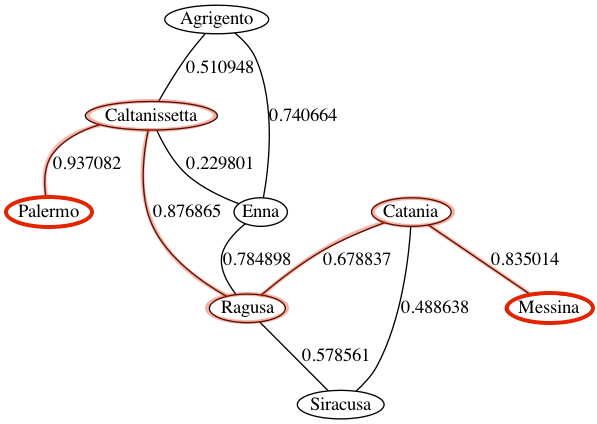
\includegraphics{imgs/shortest_path.png}

    Applications: \begin{itemize}
\item Shortest path algorithms are applied to automatically
find directions between physical locations, such as driving directions
on web mapping websites like Google Maps 
\item Considering a nondeterministic abstract machine as a graph where vertices describe
states and edges describe possible transitions, shortest path algorithms
can be used to find an optimal sequence of choices to reach a certain
goal state
\end{itemize}

    \hypertarget{bellman-ford-algorithm}{%
\section{Bellman-Ford algorithm}\label{bellman-ford-algorithm}}

The Bellman--Ford algorithm \cite{bellman-ford} is an algorithm that computes shortest paths
from a single source vertex to all of the other vertices in a
\textbf{weighted digraph}. It is slower than Dijkstra's algorithm for
the same problem, but more versatile, as it is capable of handling
graphs in which some of the edge weights are negative numbers.

    Negative edge weights are found in various applications of graphs, hence
the usefulness of this algorithm. If a graph contains a
\textbf{``negative cycle''} (i.e.~a cycle whose edges sum to a negative
value) that is reachable from the source, then there is no cheapest
path: any path that has a point on the negative cycle can be made
cheaper by one more walk around the negative cycle. In such a case, the
Bellman--Ford algorithm can detect and report the negative cycle.

    \hypertarget{first-intuition}{%
\subsection{First intuition}\label{first-intuition}}

Like Dijkstra's algorithm, Bellman--Ford proceeds by relaxation, in
which approximations to the correct distance are replaced by better ones
until they eventually reach the solution. In both algorithms, the
approximate distance to each vertex is always an overestimate of the
true distance, and is replaced by the minimum of its old value and the
length of a newly found path.

Bellman--Ford algorithm simply relaxes all the edges, \(|V|-1\) times,
where \(|V|\) is the number of vertices in the graph. In each of these
repetitions, the number of vertices with correctly calculated distances
grows, from which it follows that eventually all vertices will have
their correct distances.

    \hypertarget{toy-example}{%
\subsection{Toy Example}\label{toy-example}}
\begin{figure}[h]
\centering
\begin{tabular}{c c c}
\subfloat { 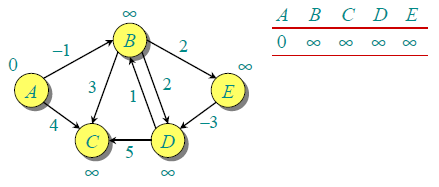
\includegraphics[scale=0.4]{imgs/bellman_0.png} }
&
\subfloat { 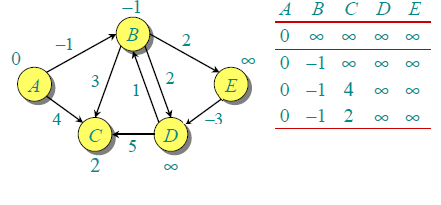
\includegraphics[scale=0.4]{imgs/bellman_1.png} }
&
\subfloat { 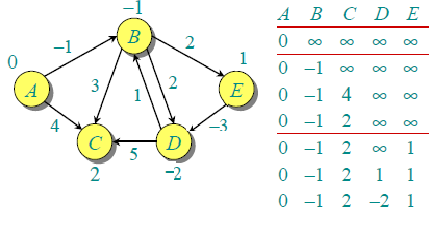
\includegraphics[scale=0.4]{imgs/bellman_2.png} }
\end{tabular}
\caption{}
\label{bellman}
\end{figure}

\begin{itemize}
\tightlist
\item
  \textbf{Iteration 0:} all distances are initialized from source vertex
  A,
\item
  \textbf{Iteration 1:} all edges are processed in the order (B,E),
  (D,B), (B,D), (A,B), (A,C), (D,C), (B,C), (E,D). Found all shortest
  paths which are at most 1 edge long,
\item
  \textbf{Iteration 2:} processing again all edges. All shortest paths
  which are at most 2 edges long are found,
\item
  \textbf{Iteration 3 and 4:} useless.
\end{itemize}

    \hypertarget{our-first-implementation}{%
\subsection{Our First Implementation}\label{our-first-implementation}}

\begin{Shaded}
\begin{Highlighting}[]
\KeywordTok{def}\NormalTok{ bellman_ford(}\VariableTok{self}\NormalTok{, source_vertex):}
\NormalTok{    vertices }\OperatorTok{=} \BuiltInTok{list}\NormalTok{(}\VariableTok{self}\NormalTok{.graph.nodes())}
    
\NormalTok{    distances }\OperatorTok{=} \BuiltInTok{dict}\NormalTok{.fromkeys(}\VariableTok{self}\NormalTok{.graph.nodes(), math.inf)}
\NormalTok{    predecessors }\OperatorTok{=} \BuiltInTok{dict}\NormalTok{.fromkeys(}\VariableTok{self}\NormalTok{.graph.nodes(), }\VariableTok{None}\NormalTok{)}
\NormalTok{    distances[source_vertex] }\OperatorTok{=} \DecValTok{0}
    \CommentTok{# relax edges}
\NormalTok{    count }\OperatorTok{=} \BuiltInTok{len}\NormalTok{(vertices) }\OperatorTok{-} \DecValTok{1}
    \ControlFlowTok{while}\NormalTok{ count }\OperatorTok{>} \DecValTok{0}\NormalTok{:}
\NormalTok{        something_has_changed }\OperatorTok{=} \VariableTok{False}
        \ControlFlowTok{for}\NormalTok{ (u, v) }\KeywordTok{in} \VariableTok{self}\NormalTok{.graph.edges():}
            \CommentTok{# considering both the symmetric edges in the form (u, v) and (v, u)}
            \ControlFlowTok{if}\NormalTok{ distances[u] }\OperatorTok{+} \BuiltInTok{float}\NormalTok{(}\VariableTok{self}\NormalTok{.graph[u][v][}\StringTok{'label'}\NormalTok{]) }\OperatorTok{<}\NormalTok{ distances[v]:}
\NormalTok{                distances[v] }\OperatorTok{=}\NormalTok{ distances[u] }\OperatorTok{+} \BuiltInTok{float}\NormalTok{(}\VariableTok{self}\NormalTok{.graph[u][v][}\StringTok{'label'}\NormalTok{])}
\NormalTok{                predecessors[v] }\OperatorTok{=}\NormalTok{ u}
\NormalTok{                something_has_changed }\OperatorTok{=} \VariableTok{True}
            \ControlFlowTok{if}\NormalTok{ distances[v] }\OperatorTok{+} \BuiltInTok{float}\NormalTok{(}\VariableTok{self}\NormalTok{.graph[v][u][}\StringTok{'label'}\NormalTok{]) }\OperatorTok{<}\NormalTok{ distances[u]:}
\NormalTok{                distances[u] }\OperatorTok{=}\NormalTok{ distances[v] }\OperatorTok{+} \BuiltInTok{float}\NormalTok{(}\VariableTok{self}\NormalTok{.graph[v][u][}\StringTok{'label'}\NormalTok{])}
\NormalTok{                predecessors[u] }\OperatorTok{=}\NormalTok{ v}
\NormalTok{                something_has_changed }\OperatorTok{=} \VariableTok{True}        
        \ControlFlowTok{if}\NormalTok{ something_has_changed }\KeywordTok{is} \VariableTok{False}\NormalTok{:}
            \ControlFlowTok{break}
\NormalTok{        count }\OperatorTok{-=} \DecValTok{1}
    \ControlFlowTok{return}\NormalTok{ distances, predecessors}
\end{Highlighting}
\end{Shaded}

    \hypertarget{computation-time}{%
\subsubsection{Computation time}\label{computation-time}}

Bellman--Ford runs in \(O(|V|\cdot |E|)\) time, where \(|V|\) and
\(|E|\) are the number of vertices and edges respectively at its worst
case.

    The Bellman--Ford algorithm may be improved in practice (although not in
the worst case), as we did, by the observation that, if an iteration of
the main loop of the algorithm terminates without making any changes,
the algorithm can be immediately terminated, as subsequent iterations
will not make any more changes. With this early termination condition,
the main loop may in some cases use many fewer than $|V|-1$
iterations, even though the worst case of the algorithm remains
unchanged.

    \hypertarget{new-strategy}{%
\subsection{New strategy}\label{new-strategy}}

The \textbf{Shortest Path Faster Algorithm (SPFA)}\cite{SPFA} is an improvement of
the Bellman--Ford algorithm which computes single-source shortest paths
in a weighted directed graph. The algorithm is believed to work well on
random sparse graphs and is particularly suitable for graphs that
contain negative-weight edges. However, the worst-case complexity of
SPFA is the same as that of Bellman--Ford, so for graphs with
nonnegative edge weights Dijkstra's algorithm is still preferred.

    The basic idea of SPFA is the same as Bellman--Ford algorithm in that
each vertex is used as a candidate to relax its adjacent vertices. The
improvement over the latter is that instead of trying all vertices
blindly, SPFA maintains a \textbf{queue} of candidate vertices and adds
a vertex to the queue only if that vertex is relaxed. This process
repeats until no more vertex can be relaxed.

    \hypertarget{our-second-implementation}{%
\subsection{Our Second Implementation}\label{our-second-implementation}}

\begin{Shaded}
\begin{Highlighting}[]
\KeywordTok{def}\NormalTok{ bellman_ford_SPFA(}\VariableTok{self}\NormalTok{, source_vertex): }
\NormalTok{    distances }\OperatorTok{=} \BuiltInTok{dict}\NormalTok{.fromkeys(}\VariableTok{self}\NormalTok{.graph.nodes(), math.inf)}
\NormalTok{    already_in_queue }\OperatorTok{=} \BuiltInTok{dict}\NormalTok{.fromkeys(}\VariableTok{self}\NormalTok{.graph.nodes(), }\VariableTok{False}\NormalTok{)}
\NormalTok{    predecessors }\OperatorTok{=} \BuiltInTok{dict}\NormalTok{.fromkeys(}\VariableTok{self}\NormalTok{.graph.nodes(), math.inf)}
\NormalTok{    distances[source_vertex] }\OperatorTok{=} \DecValTok{0}
    
\NormalTok{    q }\OperatorTok{=}\NormalTok{ deque()}
\NormalTok{    q.append(source_vertex)}
\NormalTok{    already_in_queue[source_vertex] }\OperatorTok{=} \VariableTok{True}
    \ControlFlowTok{while} \BuiltInTok{len}\NormalTok{(q) }\OperatorTok{>} \DecValTok{0}\NormalTok{:}
\NormalTok{        u }\OperatorTok{=}\NormalTok{ q.popleft()}
        \ControlFlowTok{for}\NormalTok{ (u, v) }\KeywordTok{in} \VariableTok{self}\NormalTok{.graph.edges(u):}
            \ControlFlowTok{if}\NormalTok{ distances[u] }\OperatorTok{+} \BuiltInTok{float}\NormalTok{(}\VariableTok{self}\NormalTok{.graph[u][v][}\StringTok{'label'}\NormalTok{]) }\OperatorTok{<}\NormalTok{ distances[v]:}
\NormalTok{                distances[v] }\OperatorTok{=}\NormalTok{ distances[u] }\OperatorTok{+} \BuiltInTok{float}\NormalTok{(}\VariableTok{self}\NormalTok{.graph[u][v][}\StringTok{'label'}\NormalTok{])}
                \ControlFlowTok{if} \KeywordTok{not}\NormalTok{ already_in_queue[v]:}
\NormalTok{                    q.append(v)}
\NormalTok{                    already_in_queue[v] }\OperatorTok{=} \VariableTok{True}
\NormalTok{                predecessors[v] }\OperatorTok{=}\NormalTok{ u}
            \ControlFlowTok{if}\NormalTok{ distances[v] }\OperatorTok{+} \BuiltInTok{float}\NormalTok{(}\VariableTok{self}\NormalTok{.graph[v][u][}\StringTok{'label'}\NormalTok{]) }\OperatorTok{<}\NormalTok{ distances[u]:}
\NormalTok{                distances[u] }\OperatorTok{=}\NormalTok{ distances[v] }\OperatorTok{+} \BuiltInTok{float}\NormalTok{(}\VariableTok{self}\NormalTok{.graph[v][u][}\StringTok{'label'}\NormalTok{])}
                \ControlFlowTok{if} \KeywordTok{not}\NormalTok{ already_in_queue[u]:}
\NormalTok{                    q.append(u)}
\NormalTok{                    already_in_queue[u] }\OperatorTok{=} \VariableTok{True}
\NormalTok{                predecessors[u] }\OperatorTok{=}\NormalTok{ v}
    \ControlFlowTok{return}\NormalTok{ distances, predecessors}
\end{Highlighting}
\end{Shaded}

    \hypertarget{computation-time}{%
\subsubsection{Computation time}\label{computation-time}}

The worst-case running time of the algorithm is \(O(|V|\cdot|E|)\) ,
just like the standard Bellman-Ford algorithm. However experiments
suggest that the average running time is \(O(|E|)\).

We can now compare the two strategies.

    \begin{tcolorbox}[breakable, size=fbox, boxrule=1pt, pad at break*=1mm,colback=cellbackground, colframe=cellborder]
\prompt{In}{incolor}{5}{\boxspacing}
\begin{Verbatim}[commandchars=\\\{\}]
\PY{o}{\PYZpc{}}\PY{k}{timeit} P.bellman\PYZus{}ford(\PYZdq{}Firenze\PYZdq{})
\PY{o}{\PYZpc{}}\PY{k}{timeit} P.bellman\PYZus{}ford\PYZus{}SPFA(\PYZdq{}Firenze\PYZdq{})
\end{Verbatim}
\end{tcolorbox}

    \begin{Verbatim}[commandchars=\\\{\}]
6.51 ms ± 61.5 µs per loop (mean ± std. dev. of 7 runs, 100 loops each)
2.51 ms ± 19.6 µs per loop (mean ± std. dev. of 7 runs, 100 loops each)
    \end{Verbatim}

    \begin{tcolorbox}[breakable, size=fbox, boxrule=1pt, pad at break*=1mm,colback=cellbackground, colframe=cellborder]
\prompt{In}{incolor}{6}{\boxspacing}
\begin{Verbatim}[commandchars=\\\{\}]
\PY{n}{distances}\PY{p}{,} \PY{n}{predecessors} \PY{o}{=} \PY{n}{P}\PY{o}{.}\PY{n}{bellman\PYZus{}ford\PYZus{}SPFA}\PY{p}{(}\PY{l+s+s2}{\PYZdq{}}\PY{l+s+s2}{Firenze}\PY{l+s+s2}{\PYZdq{}}\PY{p}{)}
\end{Verbatim}
\end{tcolorbox}

    \begin{tcolorbox}[breakable, size=fbox, boxrule=1pt, pad at break*=1mm,colback=cellbackground, colframe=cellborder]
\prompt{In}{incolor}{7}{\boxspacing}
\begin{Verbatim}[commandchars=\\\{\}]
\PY{n}{distances}
\end{Verbatim}
\end{tcolorbox}

            \begin{tcolorbox}[breakable, size=fbox, boxrule=.5pt, pad at break*=1mm, opacityfill=0]
\prompt{Out}{outcolor}{7}{\boxspacing}
\begin{Verbatim}[commandchars=\\\{\}]
\{'Chieti': 3.470136,
 "L'Aquila": 2.701029,
 'Pescara': 3.59269,
 'Teramo': 3.134951,
 'Matera': 7.103830000000001,
 'Potenza': 7.232769000000001,
 'Bolzano': 2.907397,
 'Catanzaro': inf,
 'Cosenza': inf,
 'Crotone': inf,
...\}
\end{Verbatim}
\end{tcolorbox}
        
    \begin{tcolorbox}[breakable, size=fbox, boxrule=1pt, pad at break*=1mm,colback=cellbackground, colframe=cellborder]
\prompt{In}{incolor}{8}{\boxspacing}
\begin{Verbatim}[commandchars=\\\{\}]
\PY{n}{predecessors}
\end{Verbatim}
\end{tcolorbox}

            \begin{tcolorbox}[breakable, size=fbox, boxrule=.5pt, pad at break*=1mm, opacityfill=0]
\prompt{Out}{outcolor}{8}{\boxspacing}
\begin{Verbatim}[commandchars=\\\{\}]
\{'Chieti': "L'Aquila",
 "L'Aquila": 'Terni',
 'Pescara': 'Chieti',
 'Teramo': "L'Aquila",
 'Matera': 'Barletta-Andria-Trani',
 'Potenza': 'Barletta-Andria-Trani',
 'Bolzano': 'Trento',
 'Catanzaro': inf,
 'Cosenza': inf,
 'Crotone': inf,
 'Reggio di Calabria': inf,
 ...\}
\end{Verbatim}
\end{tcolorbox}
       \newpage
    \hypertarget{putting-all-together}{%
\subsection{Putting all together}\label{putting-all-together}}

\begin{Shaded}
\begin{Highlighting}[]
\KeywordTok{def}\NormalTok{ bellman_ford_shortest_path(}\VariableTok{self}\NormalTok{, source_vertex, SPFA}\OperatorTok{=}\VariableTok{True}\NormalTok{):}
    \ControlFlowTok{if}\NormalTok{ SPFA:}
\NormalTok{        distances, predecessors }\OperatorTok{=} \VariableTok{self}\NormalTok{.bellman_ford_SPFA(source_vertex)}
    \ControlFlowTok{else}\NormalTok{:}
\NormalTok{        distances, predecessors }\OperatorTok{=} \VariableTok{self}\NormalTok{.bellman_ford(source_vertex)}
\NormalTok{    all__shortest_paths }\OperatorTok{=}\NormalTok{ []}
\NormalTok{    nodes }\OperatorTok{=} \BuiltInTok{list}\NormalTok{(}\VariableTok{self}\NormalTok{.graph.nodes(data}\OperatorTok{=}\VariableTok{True}\NormalTok{))}
    \ControlFlowTok{for}\NormalTok{ target_vertex }\KeywordTok{in}\NormalTok{ nodes:}
\NormalTok{        target_vertex }\OperatorTok{=}\NormalTok{ target_vertex[}\DecValTok{0}\NormalTok{]}
        \ControlFlowTok{if}\NormalTok{ predecessors[target_vertex] }\OperatorTok{==}\NormalTok{ math.inf:}
            \ControlFlowTok{continue}
        \CommentTok{# using the predecessors of each node to build the shortest path}
\NormalTok{        shortest_path }\OperatorTok{=}\NormalTok{ []}
\NormalTok{        current_node }\OperatorTok{=}\NormalTok{ target_vertex}
\NormalTok{        shortest_path.append(target_vertex)}
        \ControlFlowTok{while}\NormalTok{ current_node }\OperatorTok{!=}\NormalTok{ source_vertex:}
\NormalTok{            current_node }\OperatorTok{=}\NormalTok{ predecessors[current_node]}
            \CommentTok{# no path between the two nodes: exiting from the loop}
            \ControlFlowTok{if}\NormalTok{ current_node }\KeywordTok{is} \VariableTok{None}\NormalTok{:}
                \ControlFlowTok{break}
\NormalTok{            shortest_path.append(current_node)}
        \ControlFlowTok{if} \BuiltInTok{len}\NormalTok{(shortest_path) }\OperatorTok{!=} \DecValTok{1}\NormalTok{:}
\NormalTok{            all__shortest_paths.append(shortest_path)}
    \ControlFlowTok{return}\NormalTok{ all__shortest_paths}
\end{Highlighting}
\end{Shaded}

    The output obtained by this computation:

    \begin{tcolorbox}[breakable, size=fbox, boxrule=1pt, pad at break*=1mm,colback=cellbackground, colframe=cellborder]
\prompt{In}{incolor}{9}{\boxspacing}
\begin{Verbatim}[commandchars=\\\{\}]
\PY{n}{P}\PY{o}{.}\PY{n}{bellman\PYZus{}ford\PYZus{}shortest\PYZus{}path}\PY{p}{(}\PY{l+s+s2}{\PYZdq{}}\PY{l+s+s2}{Firenze}\PY{l+s+s2}{\PYZdq{}}\PY{p}{,} \PY{n}{SPFA}\PY{o}{=}\PY{k+kc}{True}\PY{p}{)}\PY{p}{[}\PY{p}{:}\PY{l+m+mi}{4}\PY{p}{]}
\end{Verbatim}
\end{tcolorbox}

            \begin{tcolorbox}[breakable, size=fbox, boxrule=.5pt, pad at break*=1mm, opacityfill=0]
\prompt{Out}{outcolor}{9}{\boxspacing}
\begin{Verbatim}[commandchars=\\\{\}]
[['Chieti', "L'Aquila", 'Terni', 'Perugia', 'Arezzo', 'Firenze'],
 ["L'Aquila", 'Terni', 'Perugia', 'Arezzo', 'Firenze'],
 ['Pescara', 'Chieti', "L'Aquila", 'Terni', 'Perugia', 'Arezzo', 'Firenze'],
 ['Teramo', "L'Aquila", 'Terni', 'Perugia', 'Arezzo', 'Firenze'],
 ['Matera',
  'Barletta-Andria-Trani',
  'Foggia',
  'Benevento',
  'Campobasso',
  'Chieti',
  "L'Aquila",
  'Terni',
  'Perugia',
  'Arezzo']]
\end{Verbatim}
\end{tcolorbox}
        
    \begin{tcolorbox}[breakable, size=fbox, boxrule=1pt, pad at break*=1mm,colback=cellbackground, colframe=cellborder]
\prompt{In}{incolor}{10}{\boxspacing}
\begin{Verbatim}[commandchars=\\\{\}]
\PY{o}{\PYZpc{}}\PY{k}{timeit} P.bellman\PYZus{}ford\PYZus{}shortest\PYZus{}path(\PYZdq{}Firenze\PYZdq{}, SPFA=True)
\end{Verbatim}
\end{tcolorbox}

    \begin{Verbatim}[commandchars=\\\{\}]
2.58 ms ± 30.1 µs per loop (mean ± std. dev. of 7 runs, 100 loops each)
    \end{Verbatim}

   
    \hypertarget{centrality}{%
\section{Centrality}\label{centrality}}

In network analysis, indicators of \textbf{centrality} identify the most
important vertices within a graph.
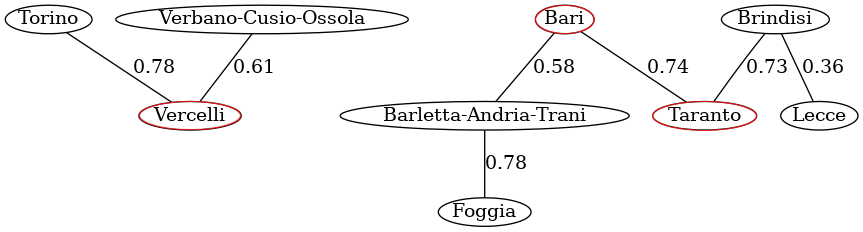
\includegraphics{./imgs/important_node.png} 
\newline
Applications: 
\begin{itemize}
\item Identifying the most influential person(s) in a social network
\item
  Key infrastructure nodes in the Internet
\item
  Super-spreaders of disease.
\end{itemize}

    \hypertarget{betweenness-centrality}{%
\section{Betweenness Centrality}\label{betweenness-centrality}}

\hypertarget{first-intuition}{%
\subsection{First intuition}\label{first-intuition}}

It was introduced as a measure for quantifying the control of a human on
the communication between other humans in a social network by
\emph{Linton Freeman}. In his conception, vertices that have a high
probability to occur on a randomly chosen \textbf{shortest path} between
two randomly chosen vertices have a high betweenness. 

    Betweenness centrality \cite{betweenneess_centrality}, in Graph Theory, is a measure of centrality in a
graph based on shortest paths. Vertices with high betweenness may have
considerable influence within a network by virtue of their control over
information passing between others. They are also the ones whose removal
from the network will most disrupt communications between other vertices
because they lie on the largest number of paths taken by messages.

    More compactly the betweenness can be represented as:

$$
g(v) =\sum\limits_{s\neq v\neq t \in V} \frac{\sigma_{st}(v)}{\sigma_{st}}
$$

where \textbf{\(\sigma_{st}\)} is total number of shortest paths from
node \(s\) to node \(t\) and \textbf{\(\sigma_{st}(v)\)} is the number
of those paths that pass through \(v\).

    \hypertarget{toy-example}{%
\subsection{Toy example}\label{toy-example}}
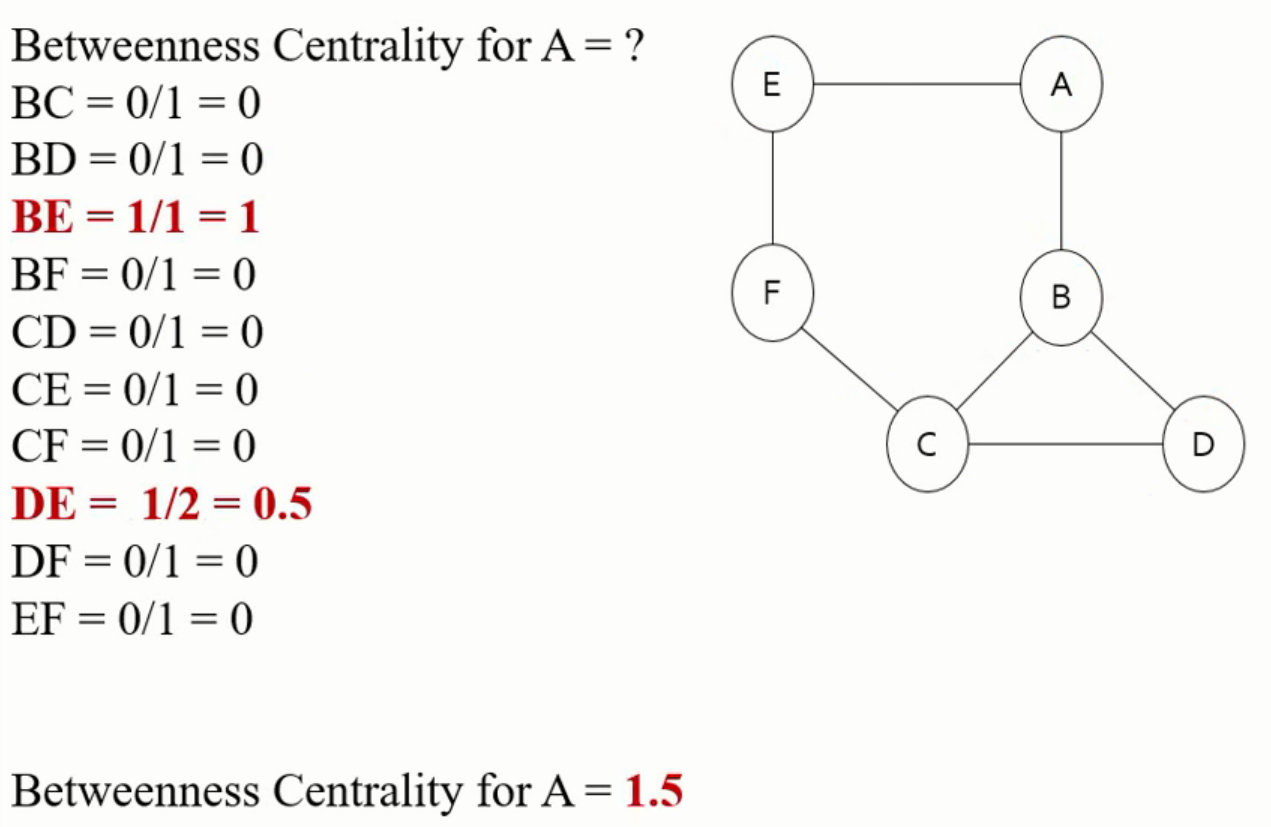
\includegraphics{./imgs/bc_toy_example.png}

    \hypertarget{betweenness-centrality-in-large-graphs}{%
\subsection{Betweenness centrality in large
graphs}\label{betweenness-centrality-in-large-graphs}}

The betweenness centrality of a node scales with the number of pairs of
nodes. Therefore, the calculation may be rescaled by dividing through by
the number of pairs of nodes not including \(v\), so that
\(g(v)\in[0,1]\). The division is done by \((N−1)(N−2)\) for directed
graphs and \(\frac{(N−1)(N−2)}{2}\) for undirected graphs, where \(N\)
is the number of nodes.

    \hypertarget{a-handy-benefit-to-betwenness-centrality}{%
\subsection{A handy benefit to betwenness
centrality}\label{a-handy-benefit-to-betwenness-centrality}}

We don't need a (fully) connected graph to calculate it
\begin{figure}[h]
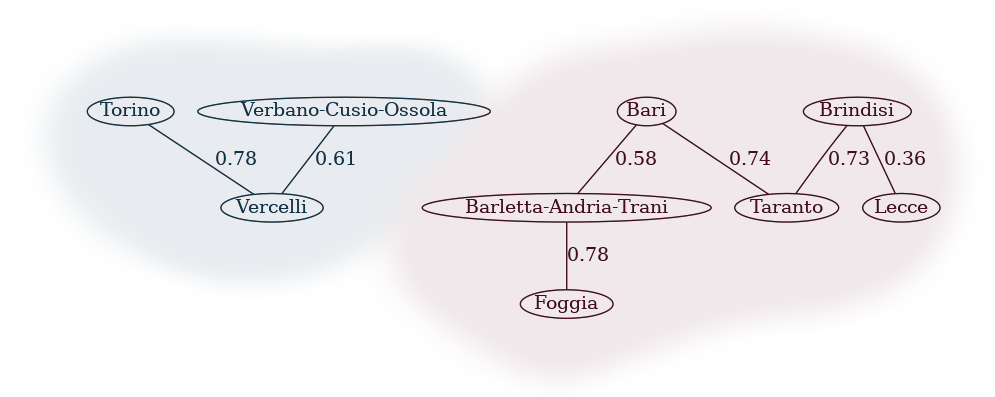
\includegraphics[scale=1]{./imgs/component.png}
\end{figure}

    \begin{tcolorbox}[breakable, size=fbox, boxrule=1pt, pad at break*=1mm,colback=cellbackground, colframe=cellborder]
\prompt{In}{incolor}{12}{\boxspacing}
\begin{Verbatim}[commandchars=\\\{\}]
\PY{n+nb}{print}\PY{p}{(}\PY{n}{P\PYZus{}toy}\PY{o}{.}\PY{n}{betweenness\PYZus{}centrality}\PY{p}{(}\PY{p}{)}\PY{p}{)}
\end{Verbatim}
\end{tcolorbox}

    \begin{Verbatim}[commandchars=\\\{\}]
\{'Torino': 0.0, 'Verbano-Cusio-Ossola': 0.0, 'Vercelli': 0.03571428571428571,
'Bari': 0.21428571428571427, 'Barletta-Andria-Trani': 0.14285714285714285,
'Brindisi': 0.14285714285714285, 'Foggia': 0.0, 'Lecce': 0.0, 'Taranto':
0.21428571428571427\}
    \end{Verbatim}

    \hypertarget{some-common-algorithms}{%
\subsection{Some common algorithms}\label{some-common-algorithms}}

Calculating the betweenness centrality of all the vertices in a graph
involves calculating the shortest paths between all pairs of vertices on
a graph, which takes:
\begin{itemize}
    \item  $\theta(|V|^3)$ for weighted graphs \emph{(Floyd--Warshall algorithm \cite{floyd_washall})}. 
    \newline $O(|V|^2 log|V| + |V||E|)$ on
sparse graphs \emph{(Johnson's algorithm \cite{jhonson} or Brandes' algorithm \cite{brandes})} 
\item $O(|V||E|)$ for unweighted graphs \emph{(Brandes' algorithm)}.
\end{itemize}

A single execution of the algorithms will find the shortest paths
between all pairs of vertices. In the last case (Brandes' algorithm) it
also calculate the betweenness value for each vertex.

    \hypertarget{our-implementation}{%
\subsection{Our implementation}\label{our-implementation}}

Here is a snippet of our implementation which calculates the betwenness
value for each node in \(O(|V|^3|E|)\). We used \emph{Bellman-Ford's
alghoritm} to find the shortest paths from a source node \(i\) to \(v\),
with \(v \in V\)

\begin{Shaded}
\begin{Highlighting}[]
\KeywordTok{def}\NormalTok{ betweenness_centrality(}\VariableTok{self}\NormalTok{, SPFA}\OperatorTok{=}\VariableTok{True}\NormalTok{):}
\NormalTok{    nodes }\OperatorTok{=} \BuiltInTok{list}\NormalTok{(}\VariableTok{self}\NormalTok{.graph.nodes(data}\OperatorTok{=}\VariableTok{True}\NormalTok{))}
\NormalTok{    N }\OperatorTok{=} \BuiltInTok{len}\NormalTok{(nodes)}
\NormalTok{    BC }\OperatorTok{=}\NormalTok{ \{nodes[i][}\DecValTok{0}\NormalTok{]: }\DecValTok{0} \ControlFlowTok{for}\NormalTok{ i }\KeywordTok{in} \BuiltInTok{range}\NormalTok{(N)\}  }
    \ControlFlowTok{for}\NormalTok{ i }\KeywordTok{in} \BuiltInTok{range}\NormalTok{(N):}
\NormalTok{        paths_lists }\OperatorTok{=} \VariableTok{self}\NormalTok{.bellman_ford_shortest_path(nodes[i][}\DecValTok{0}\NormalTok{], SPFA}\OperatorTok{=}\NormalTok{SPFA)}
        \ControlFlowTok{for}\NormalTok{ path }\KeywordTok{in}\NormalTok{ paths_lists:}
            \ControlFlowTok{for}\NormalTok{ node }\KeywordTok{in}\NormalTok{ path[}\DecValTok{1}\NormalTok{:}\OperatorTok{-}\DecValTok{1}\NormalTok{]:}
\NormalTok{                BC[node] }\OperatorTok{+=} \DecValTok{1}
    \CommentTok{# Normalize}
    \ControlFlowTok{for}\NormalTok{ i }\KeywordTok{in}\NormalTok{ BC:}
\NormalTok{        BC[i] }\OperatorTok{/=}\NormalTok{ (N }\OperatorTok{-} \DecValTok{1}\NormalTok{) }\OperatorTok{*}\NormalTok{ (N }\OperatorTok{-} \DecValTok{2}\NormalTok{)}
    \ControlFlowTok{return}\NormalTok{ BC}
\end{Highlighting}
\end{Shaded}

    \begin{tcolorbox}[breakable, size=fbox, boxrule=1pt, pad at break*=1mm,colback=cellbackground, colframe=cellborder]
\prompt{In}{incolor}{13}{\boxspacing}
\begin{Verbatim}[commandchars=\\\{\}]
\PY{o}{\PYZpc{}}\PY{k}{timeit} P.betweenness\PYZus{}centrality()
\PY{o}{\PYZpc{}}\PY{k}{timeit} nx.betweenness\PYZus{}centrality(P.graph, weight=\PYZsq{}label\PYZsq{}, normalized=True)
\PY{o}{\PYZpc{}}\PY{k}{timeit} R.betweenness\PYZus{}centrality()
\PY{o}{\PYZpc{}}\PY{k}{timeit} nx.betweenness\PYZus{}centrality(R.graph, weight=\PYZsq{}label\PYZsq{}, normalized=True)
\end{Verbatim}
\end{tcolorbox}

    \begin{Verbatim}[commandchars=\\\{\}]
241 ms ± 3.18 ms per loop (mean ± std. dev. of 7 runs, 1 loop each)
67.4 ms ± 257 µs per loop (mean ± std. dev. of 7 runs, 10 loops each)
4min 49s ± 5.22 s per loop (mean ± std. dev. of 7 runs, 1 loop each)
1min 9s ± 615 ms per loop (mean ± std. dev. of 7 runs, 1 loop each)
    \end{Verbatim}

    \hypertarget{implementation-decisions-making}{%
\section{Implementation decisions
making}\label{implementation-decisions-making}}

\begin{itemize}
\tightlist
\item
  In our implementation we used the Bellman-Ford algorithm (which is not
  good for this kind of problem) to calculate the shortest path between
  two nodes. This forced us to calculate the shortes path in both
  directions, therefore we needed to divide by 2 the result of the
  betweenness of the considered node. We have calculated all the
  shortest paths in the graph in \(O(|V|^2|E|)\) while Johnson's
  algorithm takes \(O(|V|^2 log|V| + |V||E|)\)
\end{itemize}

    \begin{itemize}
\tightlist
\item
  Due to the great precision of the distances between the various nodes
  (graph \textbf{P} and \textbf{R}) and for the definition of the
  Bellman-Ford's algorithm itself, we thought it was appropriate to
  simplify the algorithm assuming that there could be at most one
  shortest path between each pair of nodes.
\end{itemize}

    \begin{tcolorbox}[breakable, size=fbox, boxrule=1pt, pad at break*=1mm,colback=cellbackground, colframe=cellborder]
\prompt{In}{incolor}{14}{\boxspacing}
\begin{Verbatim}[commandchars=\\\{\}]
\PY{n+nb}{print}\PY{p}{(}\PY{l+s+s2}{\PYZdq{}}\PY{l+s+s2}{Our Implementation: }\PY{l+s+s2}{\PYZdq{}}\PY{p}{,}\PY{n+nb}{list}\PY{p}{(}\PY{n}{P}\PY{o}{.}\PY{n}{betweenness\PYZus{}centrality}\PY{p}{(}\PY{p}{)}\PY{o}{.}\PY{n}{items}\PY{p}{(}\PY{p}{)}\PY{p}{)}\PY{p}{[}\PY{l+m+mi}{0}\PY{p}{:}\PY{l+m+mi}{3}\PY{p}{]}\PY{p}{)}
\PY{n+nb}{print}\PY{p}{(}\PY{l+s+s2}{\PYZdq{}}\PY{l+s+se}{\PYZbs{}n}\PY{l+s+se}{\PYZbs{}n}\PY{l+s+s2}{Networkx method: }\PY{l+s+s2}{\PYZdq{}}\PY{p}{,}\PY{n+nb}{list}\PY{p}{(}\PY{n}{nx}\PY{o}{.}\PY{n}{betweenness\PYZus{}centrality}\PY{p}{(}\PY{n}{P}\PY{o}{.}\PY{n}{graph}\PY{p}{,} \PY{n}{weight}\PY{o}{=}\PY{l+s+s1}{\PYZsq{}}\PY{l+s+s1}{label}\PY{l+s+s1}{\PYZsq{}}\PY{p}{)}\PY{o}{.}\PY{n}{items}\PY{p}{(}\PY{p}{)}\PY{p}{)}\PY{p}{[}\PY{l+m+mi}{0}\PY{p}{:}\PY{l+m+mi}{3}\PY{p}{]}\PY{p}{)}
\end{Verbatim}
\end{tcolorbox}

    \begin{Verbatim}[commandchars=\\\{\}]
Our Implementation:  [('Chieti', 0.19748427672955976), ("L'Aquila",
0.06037735849056604), ('Pescara', 0.005750224618149146)]


Networkx method:  [('Chieti', 0.19748427672955976), ("L'Aquila",
0.06037735849056604), ('Pescara', 0.005750224618149146)]
    \end{Verbatim}

    \begin{itemize}
\tightlist
\item
  Due to the large number of nodes we normalized the value of the
  betweenness so that \(g(v)\in[0,1]\). The division is done by
  \(\frac{(N−1)(N−2)}{2}\) cause we are working with an undirected
  graph.
\end{itemize}

    \begin{itemize}
\tightlist
\item
  Based on the considerations made, the final formula for calculating
  the betweenness centrality of a node \(v\) is

  \(g(v) =\frac{\sum\limits_{s\neq v\neq t \in V} \frac{\sigma_{st}(v)}{\sigma_{st}}}{2}\frac{2}{(N-1)(N-2)} = \frac{\sum\limits_{s\neq v\neq t \in V} \frac{\sigma_{st}(v)}{\sigma_{st}}}{(N-1)(N-2)}\)

  where \(\sigma_{st}(v)\), \(\sigma_{st} \in \{0,1\}\).
\end{itemize}


\printbibliography[
heading=bibintoc,
title={Bibliography}]    
\end{document}

